%!TEX root = proj_report_outline.tex
\chapter{Background \& Related Work}\label{background}

This chapter aims to provide background on the innovation ecosystem and contextualise where in this landscape PitchHub fits in. First, this chapter introduces the concept of an innovation community, and explores the roles that are present within this community. Second, this chapter discusses innovation online and what security issues are raised in this environment. Third, this chapter describes the current collaborative platforms being used in the innovation space and establishes where each stands within the role taxonomy. 

\section{Innovation Community}
In this world of constant communication the creation of ideas is an activity no longer isolated to inventors or researchers. It has evolved into what can instead be seen as a collaborative effort from a diverse community of actors. Von Hippel defined innovation communities as ``nodes consisting of individuals or firms interconnected by information transfer links which may involve face-to-face, electronic, or other communication'' \cite{von2005democratizing}. The world of innovation today now includes actors from increasingly disparate domains who are able to contribute their unique capabilities to the innovation process \cite{che2003optimal}. The influx of unique skills being mixed into the innovation community has resulted in more unique opportunities for innovation being made possible. To take advantage of these opportunities it is critical that there be a communication layer where these actors may collaborate.

\section{Common Roles in Innovation}\label{commonRolesInInnovation}

The process of driving an idea from its conceptualisation to its realisation commonly requires a variety of actors. These actors as a team bring together the knowledge, skills and resources required to action the idea's fulfilment \cite{engelberger1982robotics}. For example, the Apple ][ came to being with Steve Wozniak providing the technical knowledge and skills, Steve Jobs providing the project goals and marketing drive, and Mike Markulla providing the resources to finance the operation \cite{livingston2007founders}. This is a recurring pattern, where subgroups of a team producing an innovative product or service have different responsibilities in regards to the end product or service's realisation. To formalise these common responsibilities Callaghan Innovation has identified four distinct roles that are embodied within the innovation process:

\begin{itemize}
	\item Challenger
	\item Enabler
	\item Solver
	\item Facilitator
\end{itemize}

Challengers provide the idea or problem to be solved in order to realise a business opportunity. Enablers provide the resources required to action innovation, this may be in terms of man-power, assets or financing. Solvers contribute answers to the idea or problem presented by the Challenger(s). Facilitators provide the connections to drive the innovation's execution, this may be in terms of connecting the idea to other people or helping the idea gain visibility. In most cases these roles are too large for one person to embody them all. To continue with the Apple ][ example, Steve Jobs may be categorised as a Challenger, asking why computers can't serve the consumer market, Steve Wozniak can be seen as an Enabler and Solver, as he both designed and built the Apple ][, and Mike Markulla, can be regarded as an Enabler and Facilitator, as he financed the production and also lent his reputation to the product. It is important to recognise that many innovations, such as the Apple ][, require a collaboration between these roles to be successfully executed. Platforms seeking to encourage innovation must therefore provide functionality for the collaboration/networking between actors fulfilling these roles.

\section{Innovation Online}
Since the advent of the world wide web communication and knowledge sharing has never been more accessible or easy. Naturally, this has been a boon for the innovation community. The reach the world wide web affords enables innovation communities to capitalise on sources of innovative potential and knowledge at unprecedented scale \cite{hautz2010establish}.

\section{Security, Privacy, and Trust in Online Communities}

The nature of bringing the innovation process online consequently involves bringing what could be commercially sensitive information online also. Given this reality, there is a large amount of trust involved where users are relying on the platforms they are inputting their sensitive data into to take precautions to keep this data safe. \citeauthor{boyd2002community}'s research into online marketplaces has shown the importance of this trust in a business context: ``without trust, risk is paralyzing; transactions simply do not take place'' \cite{boyd2002community}. This notion is similarly applicable in the online innovation space, the only difference being that users are transacting in intellectual property and skills rather than money. Because users have very little power over how their data is stored and disseminated it is paramount for platforms to make good on this trust. This can be achieved by implementing safeguards against security threats and providing functionality that gives users {\em control} over the visibility/dissemination of their data.

Unfortunately, the security of online communities does not solely depend on their technical security. As explored by \citeauthor{johnson2012facebook} in their work regarding online privacy \cite{johnson2012facebook}, social networks also face the problem of managing insider threat. Insider threat is where users unintentionally share content with members on the network. This problem is raised by the lack of or under use of privacy controls. In a platform where commercially sensitive information is the content at stake it is important that the platform enforce (or encourage) the use of these privacy controls. A study conducted by \citeauthor{shin2010effects} explores the constructs of security, privacy, and trust in social networks, his findings affirmed the above discussion, concluding that security and privacy play vital roles in developing trust from the users \cite{shin2010effects}.

\section{Related Work}

This section explores the current solutions being used to facilitate collaboration in the innovation community. This is done through the use of the Innovation Role Taxonomy developed. The Innovation Role Taxonomy consists of the roles identified in Section \ref{commonRolesInInnovation} as well as their level of support for collaboration between roles: either implicit or explicit. Implicit support is characterised by users using a system to support collaboration despite this not being the system's intended use.
\\
\newline
\textbf{IdeaForge} \cite{ideaForge:online}
is a collaborative innovation platform that explicitly supports collaboration between the Challenger, Enabler and Solver roles. In it's own parlance IdeaForge is described as a three-sided marketplace where users can provide ``ideas, time/skills or cash/resources". The main aim for this platform is to facilitate any-time/anywhere collaboration within the global innovation community. Additionally, IdeaForge provides some visibility settings for ideas such that they may be scoped as ``visible publicly'' or ``members only''. IdeaForge does not provide explicit support for the Facilitator role, therefore ideas being hosted on IdeaForge require external facilitation. IdeaForge can be regarded as the most similar to PitchHub in spirit as it serves many of the roles identified and provides scoping functionality.
\\
\newline
\textbf{Assembly} \cite{assembly:online}
is a collaborative platform that implicitly supports Challenger, Enabler, Solver, and Facilitator roles. The implicit collaboration support is facilitated through it's forum-like structure, where any of these roles may contribute and network. This is adequate however as established in \citeauthor{hautz2010establish}'s study of online innovation communities, they point out that innovation communities have a ``very specific purpose and therefore requires a special kind of user participation and interaction'' \cite{hautz2010establish}, this is why explicit support of collaboration between these roles is preferred over implicit support. Important to note is that Assembly is organised around groups rather than ideas, however these groups may be working on one or more ideas. Assembly's recommender system functionality, where users get recommended groups they may be interested in, illustrates how Assembly itself can be seen as carrying out the Facilitator's role. PitchHub and Assembly differ on focus, where PitchHub focuses on the idea Assembly focuses on the groups, this structure while applicable to the innovation space is less directed towards the immediate fulfilment of ideas and more for general collaboration.
\\
\newline
\textbf{AngelList} \cite{Angel:online} and \textbf{Enterprise Angels} \cite{enterpriseAngles:online} are examples of online platforms for investors (a subset of of Enablers) looking to fund businesses. Crowd funding and microequity platforms such as \textbf{Kickstarter} \cite{Kicks6:online}, \textbf{Indiegogo} \cite{Indie3:online} and \textbf{PledgeMe} \cite{Pledge:online} are becoming increasingly viable sources of funding for innovation. These platforms are primarily for Solvers looking to seed their solutions, and Enablers looking to get return on their investments. An interesting phenomenon of these platforms is the social ``hype" that is sometimes garnered around many of the products/services launched on these platforms. While the solicitation of funds is not a primary goal of PitchHub the inherent socialness of these funding platforms is directly comparable.
\\
\newline
Inevitably large social networks have also been used in the innovation space as platforms to help facilitate collaboration. Examples include \textbf{LinkedIn} \cite{Linkedin:online} being used by New Zealand Healthcare Innovation \cite{nzHealthCare:online}, \textbf{Facebook} \cite{Faceb6:online} being used in the Great New Zealand Science Project \cite{greatNZScience:online}, and \textbf{Google Groups} \cite{Googlegroups:online} being used in the National Science Challenges \cite{nzNSC10:online}. These platforms have the inherent benefit of convenience as many people in the innovation ecosystem are already members of these networks. Beyond the lack of explicit support for collaboration between the roles identified in Section \ref{commonRolesInInnovation} these platforms also suffer from lack of (used) privacy controls. This leads to what is not a conducive environment for users wishing to discuss commercially sensitive information. These re-purposed examples of social networks are in stark contrast to PitchHub's goal of facilitating collaborative innovation in a directed and secure manner.
\\
\newline
Overall, the proliferation of online networks has been a boon for communities, enabling unprecedented reach. The innovation community is no different and has benefited greatly from these networks, however as demonstrated in the above investigation these networks lack features which serve the directed collaboration between roles within the innovation community.

\section{Innovation Role Taxonomy}

TODO

This is most evident through the Innovation Role Taxonomy, Fig \ref{fig:collaborative_platforms}. It is clear that there is a need for PitchHub, or a similar service, where explicit support for collaboration between all roles is provided.

\begin{figure}[ht]
    \centering
    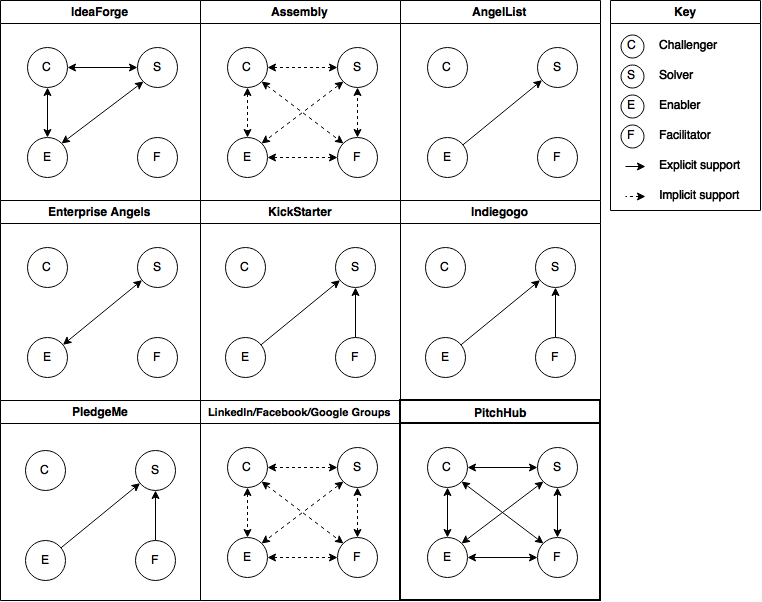
\includegraphics[width=1\textwidth]{collaborative_platforms}
    \caption{All collaborative platforms investigated do not provide explicit collaboration support between the all roles identified in Section \ref{commonRolesInInnovation}. PitchHub aims to fix this by supporting networking between all roles. }
    \label{fig:collaborative_platforms}
\end{figure}
